\documentclass[a4paper,12pt]{article}
\usepackage[T2A]{fontenc}
\usepackage[utf8]{inputenc}
\usepackage[english,russian]{babel}
\tolerance 500
\usepackage{mathtext}
\usepackage{ascii}
\usepackage{indentfirst}
\usepackage{graphicx}
\usepackage{float}
\graphicspath{{images/}}
% use hyperlinks
\usepackage[breaklinks]{hyperref}
\hypersetup{
  unicode=true,
  pdfborder={0 0 0}
}

\usepackage[a4paper]{geometry}
\geometry{left=2cm}
\geometry{right=2cm}
\geometry{top=2cm}
\geometry{bottom=2cm}

\begin{document}
\newgeometry{left=1cm,right=1cm,bottom=2cm,top=2cm}
{
\thispagestyle{empty}
\newpage

\begin{center}
ФЕДЕРАЛЬНОЕ ГОСУДАРСТВЕННОЕ ОБРАЗОВАТЕЛЬНОЕ УЧРЕЖДЕНИЕ ВЫСШЕГО ПРОФЕССИОНАЛЬНОГО ОБРАЗОВАНИЯ \\
\vspace{1cm}
САНКТ-ПЕТЕРБУРГСКИЙ ГОСУДАРСТВЕННЫЙ УНИВЕРСИТЕТ \\*
ВОДНЫХ КОММУНИКАЦИЙ \\*
\hrulefill\\
\textbf{Факультет информационных технологий \\
Кафедра вычислительных систем и информатики \\}
\end{center}

\vfill

\begin{center}
\textbf{Руководство}\\
\medskip
по развертыванию сервера на платформе\\
\medskip
\end{center}

\begin{center}
\textbf{Windows Server 2008 R2, Novell Open Enterprise Server 2}\\
\end{center}

\vfill
\vfill

\begin{center}
Санкт-Петербург \number\year
\end{center}
\clearpage

}
\restoregeometry
\tableofcontents
\newpage

\phantomsection
\addcontentsline{toc}{section}{Введение}
\section*{Введение}
В этом пособии рассматриваются основы администрирования компьютерных сетей на базе операционных систем Microsoft Windows Server 2008 R2 и Novell Open Enterprise Server 2, начиная с установки, заканчивая настойкой базовых служб раздачи сетевых адресов, разрешения имён, управления пользователями. Наша задача состоит в том, чтобы показать, что можно решать схожие задачи администрирования на принципиально разных операционных системах. В результате получатся два сервера с одинаковым функционалом, достаточным для решения повсеневных задач небольшой фирмы.
\par
Мы рассмотрим такие задачи как:
\begin{itemize}
\item установка сервера (Windows Server 2008 R2/Novell Open Enterprise Server 2);
\item настройка службы DHCP;
\item настройка службы DNS;
\item настройка Active Directory/eDirectory;
\item создание перемещаемых профилей;
\item демонстрация рабочего процесса.
\end{itemize}
\par
Все правки, предложения и замечания Вы можете оставить здесь: \url{http://github.com/4e6/study-admin-guide/issues} или написать их нам на адрес \href{mailto:suwcag@gmail.com}{suwcag@gmail.com}.
\cleardoublepage
%\setcounter{section}{0}
\part{Windows Server 2008 R2}
\thispagestyle{plain}
Операционная система \foreignlanguage{english}{Windows Server 2008 R2}, созданная на основе \foreignlanguage{english}{Windows Server 2008}, расширяет базовые возможности операционной системы \foreignlanguage{english}{Windows Server} и предоставляет новые мощные средства, помогая организациям всех размеров повышать управляемость, доступность и гибкость в соответствии с изменяющимися требованиями бизнеса.
Как и Windows 7, Windows Server 2008 R2 использует ядро Windows NT 6.1.
Новые возможности включают улучшенную виртуализацию, новую версию \foreignlanguage{english}{Active Directory Internet Information Services 7.6} и поддержку до 256 процессоров. Система доступна только в 64-разрядном варианте.
\foreignlanguage{english}{Text in language B. This environment switches all language-related definitions, like the language specific names for figures, tables etc. to the other language.}

\section{Получение дистрибутива}
Система \textit{Windows Server 2008 R2} является платным серверным решением корпорации \textit{Microsoft}, получить ознакомительный дистрибутив можно на странице \textit{центра пробного програмного обеспечения TechNet}\footnote{http://technet.microsoft.com/ru-ru/evalcenter/} портала \textit{Microsoft TechNet}.

\section{Выбор выпуска}
\textit{Windows Server 2008 R2} поставляется в нескольких редакциях, приведем сравнительную таблицу версий основанную на ролях сервера:
\begin{figure}[H]
\center{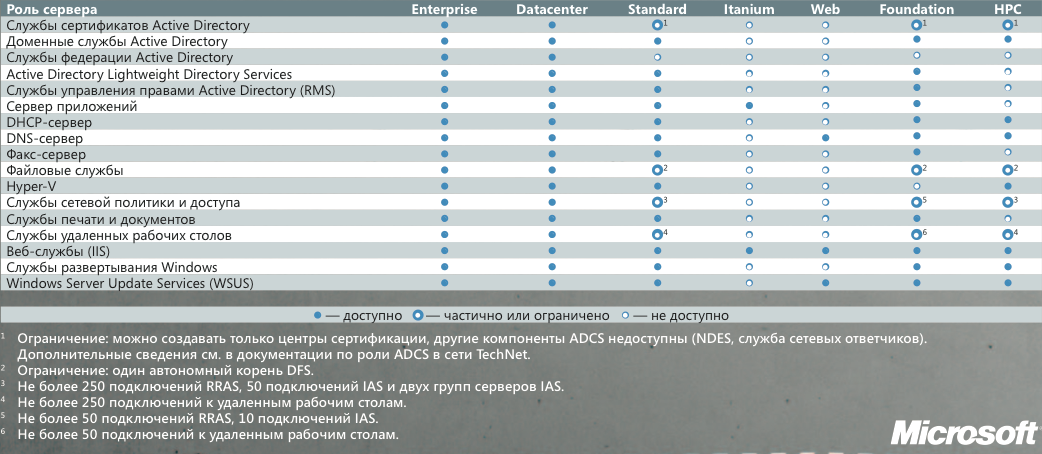
\includegraphics[width=1\linewidth]{ws2k8/diff.png}}
\end{figure}
Как мы видим для наших целей(AD, DNS, DHCP) подойдет выпуск \textit{Standard}.
\newpage
\section{Установка}
Для начала установки загружаемся с установочного диска и настраиваем языковые настройки:
\begin{figure}[H]
\center{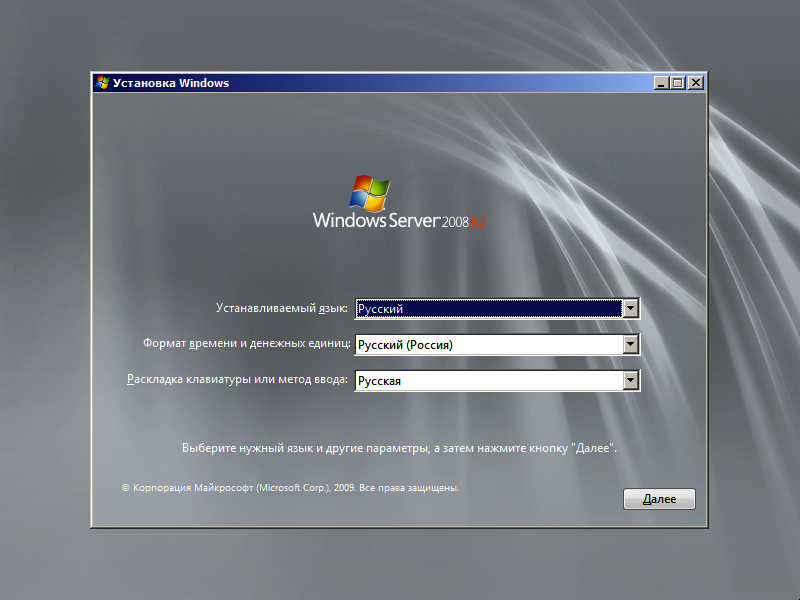
\includegraphics[width=1\linewidth]{ws2k8/install_1.png}}
\caption{Окно языковых настроек}
\label{igas1}
\end{figure}
\clearpage
Для того чтобы приступить к установке, жмем кнопку \textit{Установить}.
\begin{figure}[H]
\center{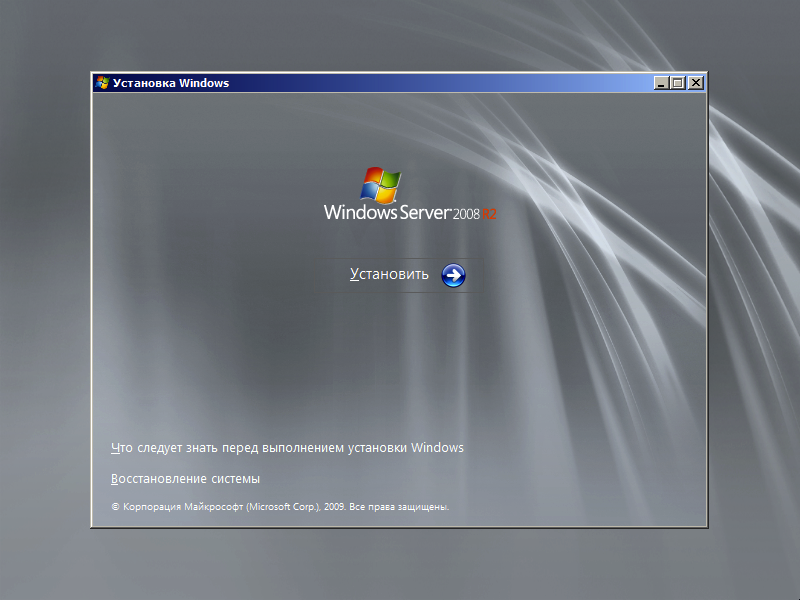
\includegraphics[width=1\linewidth]{ws2k8/install_2.png}}
\caption{Окно начала установки}
\label{igas2}
\end{figure}
\clearpage
Как мы уже решили, мы будем устанавливать версию \textit{Standard} полную, т.к. вариант установки \textit{Server Core} подразумевает минимальную установку и управление из командной строки, этот вариант рассчитан на более опытных пользователей и хуже подходит для обучения.
\begin{figure}[H]
\center{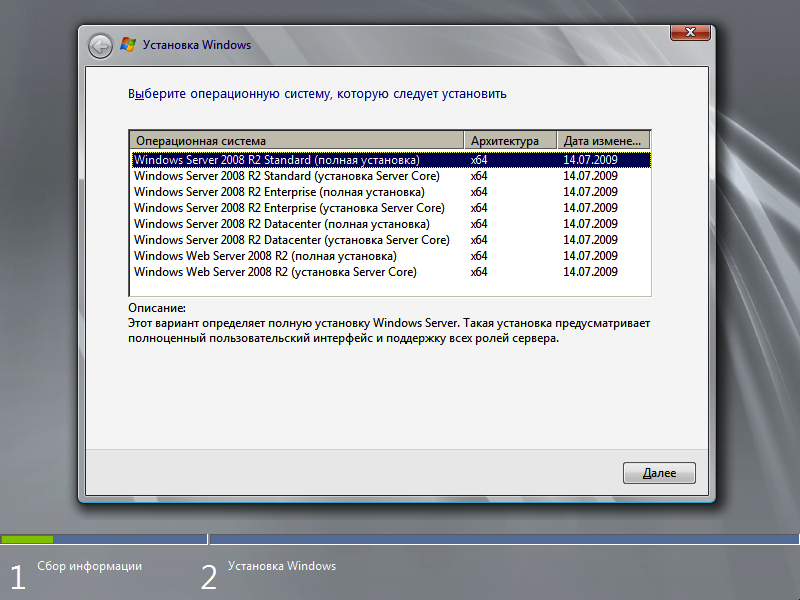
\includegraphics[width=1\linewidth]{ws2k8/install_3.png}}
\caption{Окно выбора редакции}
\label{igas3}
\end{figure}
\clearpage
Ознакомтесь с лицензионным соглашением и если согласны то отметьте соответствующий пункт меню и переходите к следующему шагу.
\begin{figure}[H]
\center{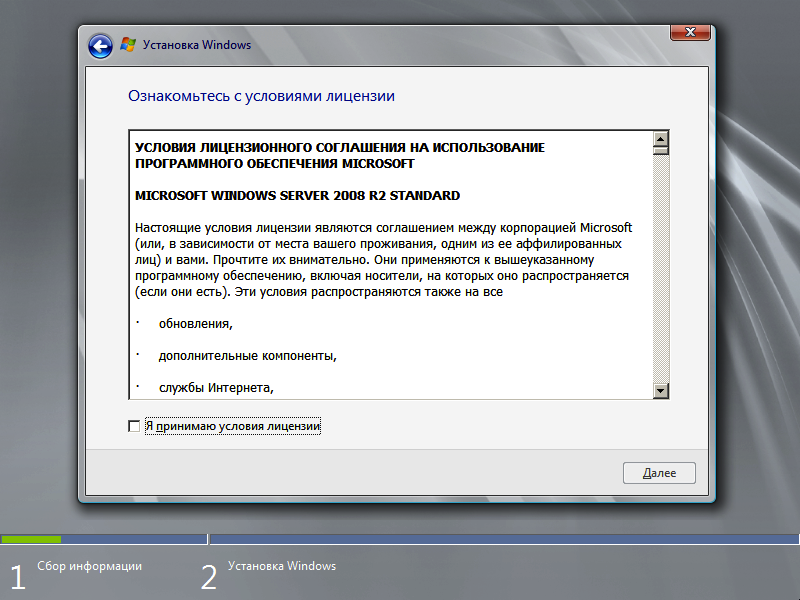
\includegraphics[width=1\linewidth]{ws2k8/install_4.png}}
\caption{Окно лицензионного соглашения}
\label{igas4}
\end{figure}
\clearpage
Выбираем пункт \textit{<<полная установка>>}, т.к. подразумевается что мы настраиваем новый сервер, а обновление существующего сервера выходит за рамки данного пособия.
\begin{figure}[H]
\center{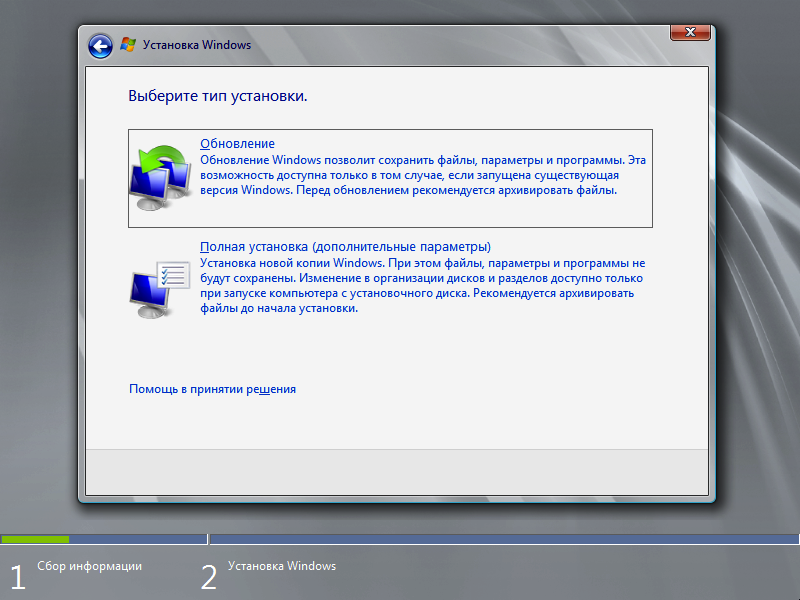
\includegraphics[width=1\linewidth]{ws2k8/install_5.png}}
\caption{Окно способа установки}
\label{igas5}
\end{figure}
\clearpage
У нас не стоит задачи создания резервного копирования данных, поэтому мы можем использовать один локальный диск.
\begin{figure}[H]
\center{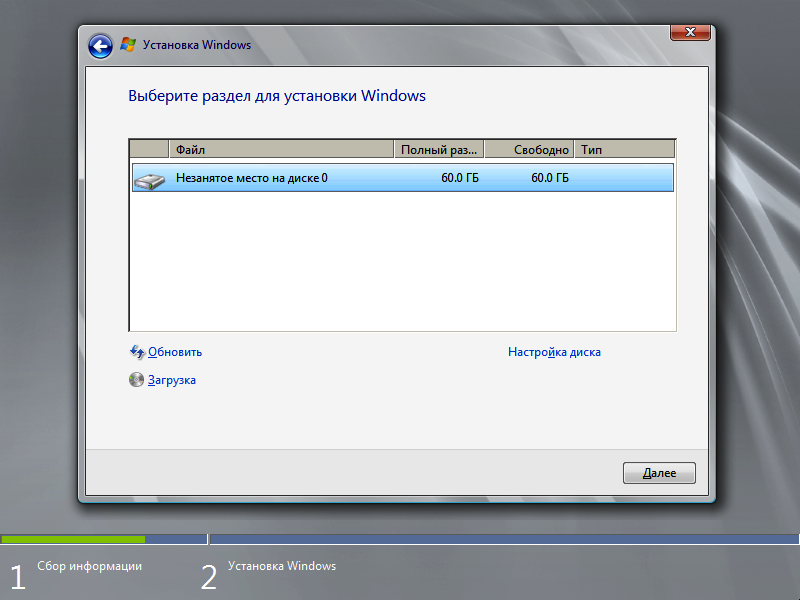
\includegraphics[width=1\linewidth]{ws2k8/install_6.png}}
\caption{Окно разметки диска(ов)}
\label{igas6}
\end{figure}
\clearpage
Ожидаем окончания копирования/распаковки файлов и установки компонентов/обновлений.
\begin{figure}[H]
\center{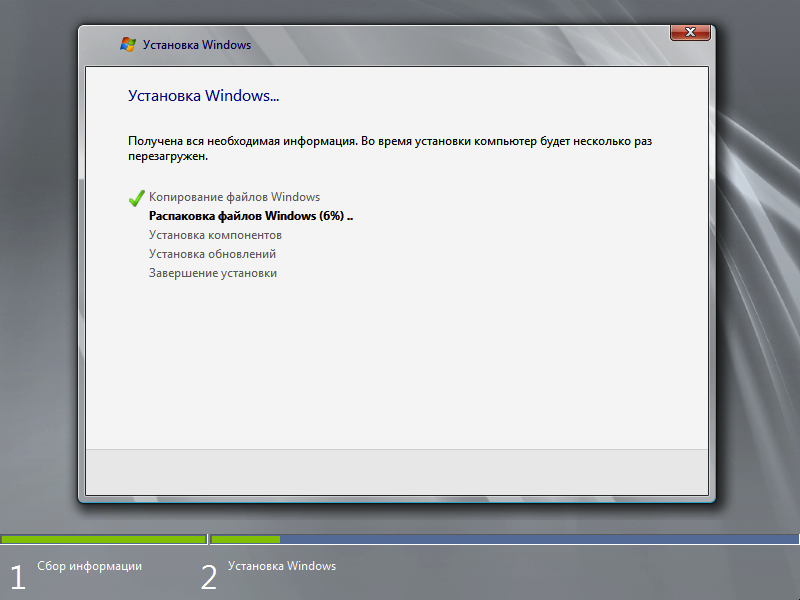
\includegraphics[width=1\linewidth]{ws2k8/install_7.png}}
\caption{Окно установки}
\label{igas7}
\end{figure}
\clearpage
По окончании установки мы увидим окно предупреждения о необходимой перезагрузке.
\begin{figure}[H]
\center{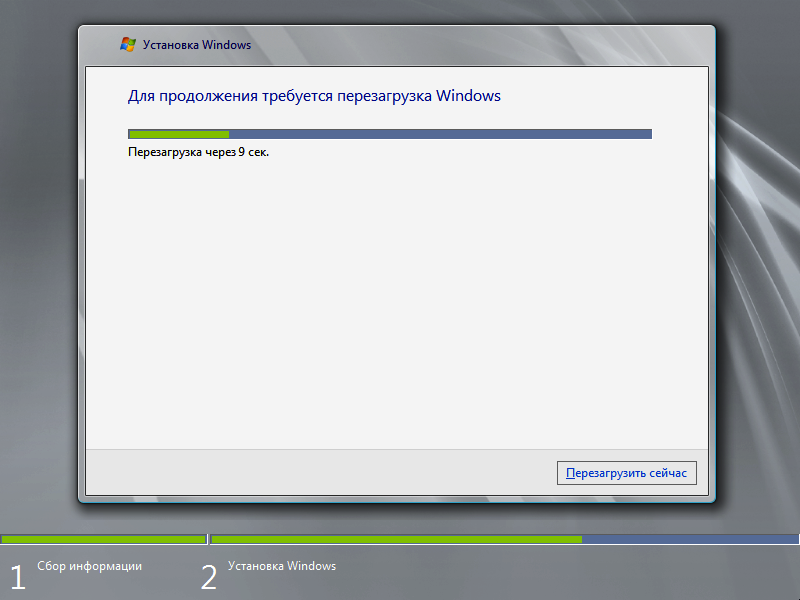
\includegraphics[width=1\linewidth]{ws2k8/install_8.png}}
\caption{Окно перезагрузки}
\label{igas8}
\end{figure}
\clearpage
Завершающий этап установки.
\begin{figure}[H]
\center{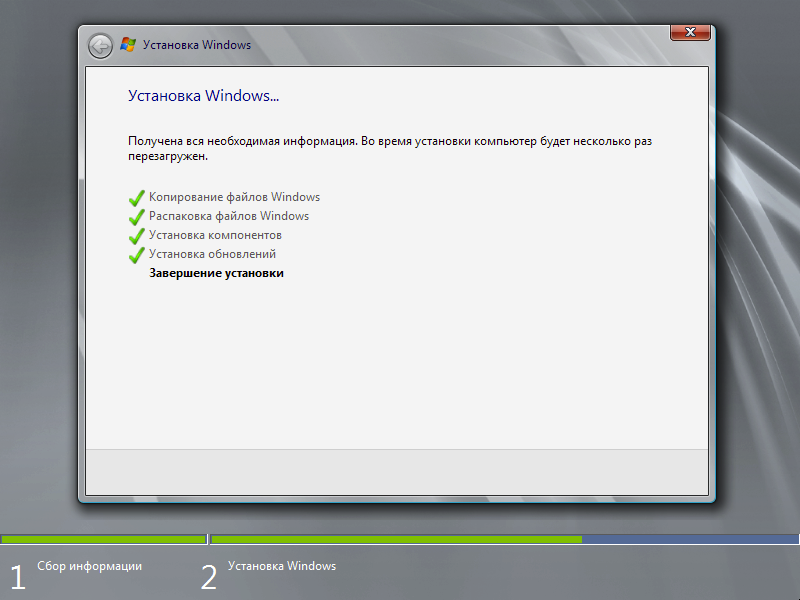
\includegraphics[width=1\linewidth]{ws2k8/install_9.png}}
\caption{Окно завершения установки}
\label{igas9}
\end{figure}
\clearpage
После завершения установки мы увидим предупреждение о необходимости смены пароля администратора.
\begin{figure}[H]
\center{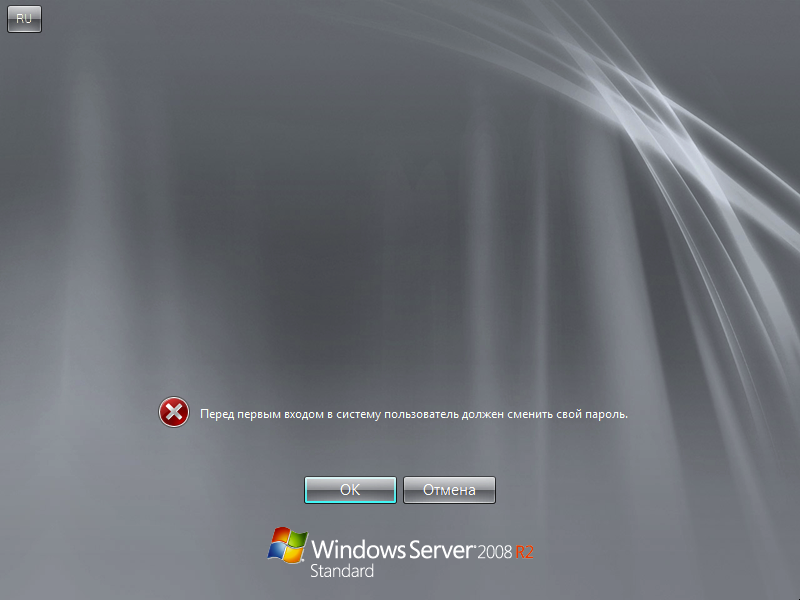
\includegraphics[width=1\linewidth]{ws2k8/install_10.png}}
\caption{Предупреждение}
\label{igas10}
\end{figure}
\clearpage
Последним этапом перед запуском системы является задание пароля для администратора.
\begin{figure}[H]
\center{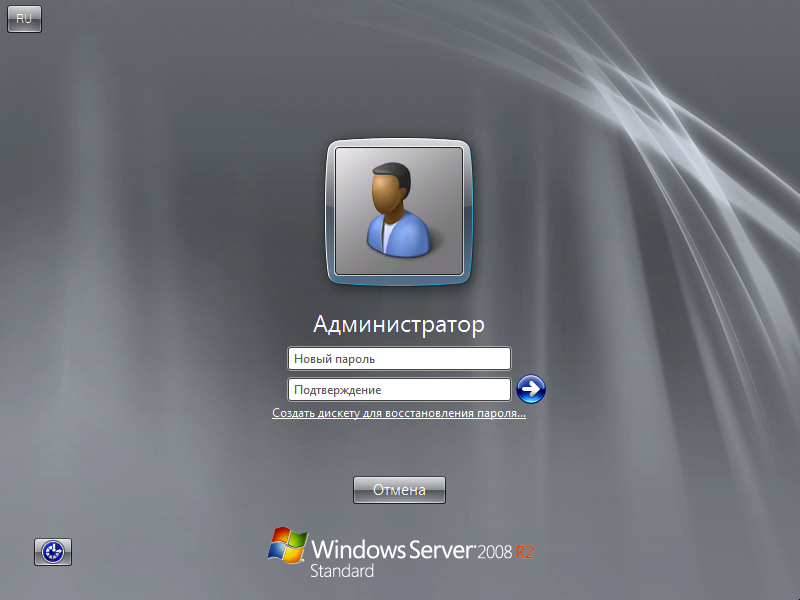
\includegraphics[width=1\linewidth]{ws2k8/install_11.png}}
\caption{Форма смены пароля}
\label{igas11}
\end{figure}

\section{Настройка}
\subsection{Предварительная настройка}
\begin{figure}[H]
\center{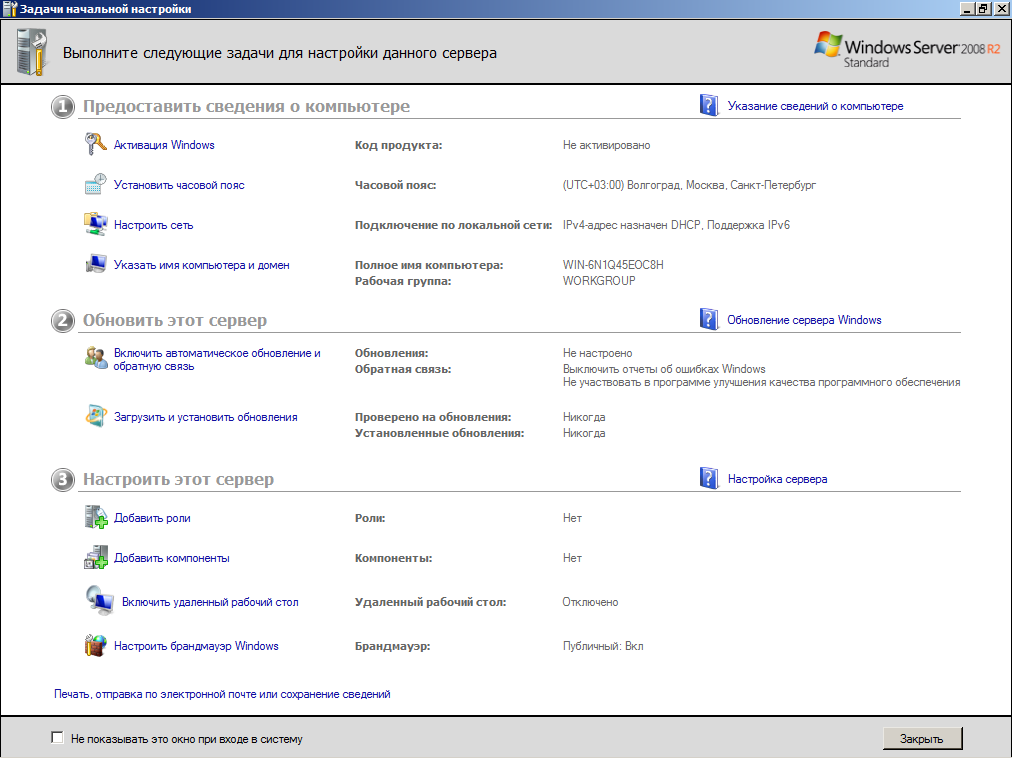
\includegraphics[width=1\linewidth]{ws2k8/setup_1.png}}
\caption{Окно задач начальной настройки}
\label{igas12}
\end{figure}
Начнем с настройки сети, перейдем в раздел \textit{Настроить сеть} и зайдем в свойства нашего подключения.
\begin{figure}[H]
\center{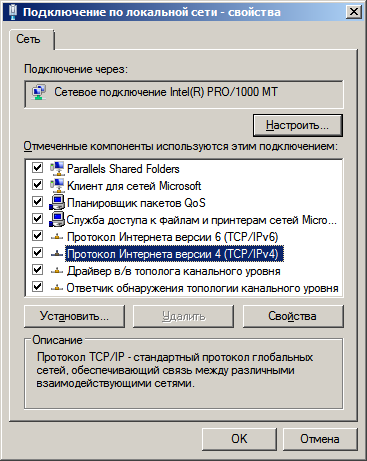
\includegraphics{ws2k8/setup_2.png}}
\caption{Окно задач начальной настройки}
\label{igas13}
\end{figure}
Отключим \textit{Протокол Интернета версии 6 (TCP/IPv6)}, затем выберем \textit{Протокол Интернета версии 4 (TCP/IPv4)} и кликнув по кнопке \textit{Cвойства} настроим наше подключение как показанно на рисунке \ref{igas14}.
\begin{figure}[H]
\center{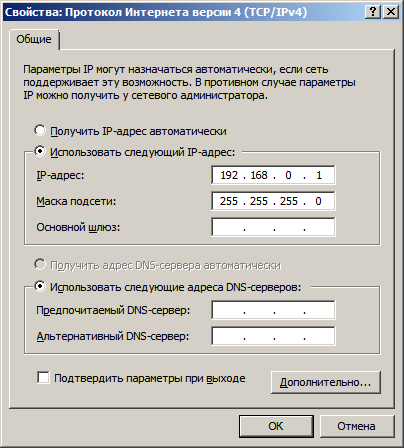
\includegraphics[scale=1]{ws2k8/setup_3.png}}
\caption{Окно задач начальной настройки}
\label{igas14}
\end{figure}
Укажем имя нашего компьютера, для этого нажмем \emph{Указать имя компьютера и домен}, а затем на кнопку \emph{Изменить...}, в поле \emph{Имя компьютера} впишем \texttt{server}, применим изменения и перезагрузимся.
\par
Также следует настроить автоматическое обновление системы, чтобы Ваш сервер был более защищен. Перейдем в раздел \textit{Включить автоматическое обновление и обратную связь}, его можно найти в \textit{Задачах начальной настройки} (рис.~\ref{igas12}). В появившемя окне выбираем \textit{Включить автоматическое обновление Windows и сбор отзывов и предложений}. После этого первоначальную проверку сделаем вручную чтобы не ждать пока это сделает систем по расписанию. Перейдем в раздел \textit{Загрузить и установить обновления} и нажмем на кнопку \textit{Проверка обновлений}, а после как система проверит наличие обновлений нажимаем кнопку \textit{Установить обновления}.
\newpage
\subsection{DHCP}
Приступим к добавлению первой роли нашего сервера -- DHCP. Из \textit{окна начальной настройки} (рис.~\ref{igas12}) в разделе \textit{Настроить этот сервер} нажмем на \textit{Добавить роли}.
\par
В окне \textit{мастера добавления ролей} нажимаем \textit{далее}, чтобы пропустить раздел \textit{Перед началом работы}, и увидим раздел \textit{Выбор ролей сервера} (рис.~\ref{igas16}), отметим \textit{DHCP-сервер} и нажмем \textit{Далее}, увидим описание роли и еще раз нажмем \textit{Далее}.
\begin{figure}[H]
\center{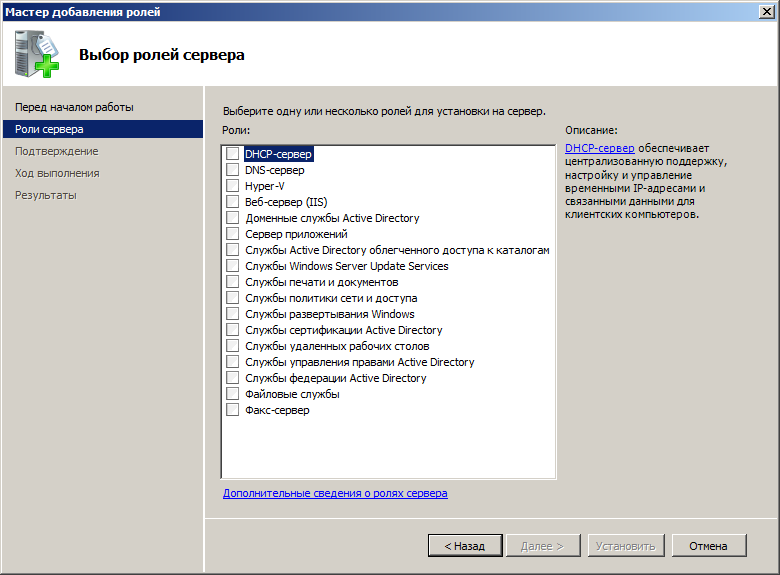
\includegraphics[scale=0.6]{ws2k8/dhcp_2.png}}
\caption{Выбор ролей сервера}
\label{igas16}
\end{figure}
В разделе \textit{Выбор привязки сетевого подключения} (рис.~\ref{igas18}) проверяем чтобы был отмечен только IP нашего внутреннего интерфейса и жмем \textit{далее}.
\begin{figure}[H]
\center{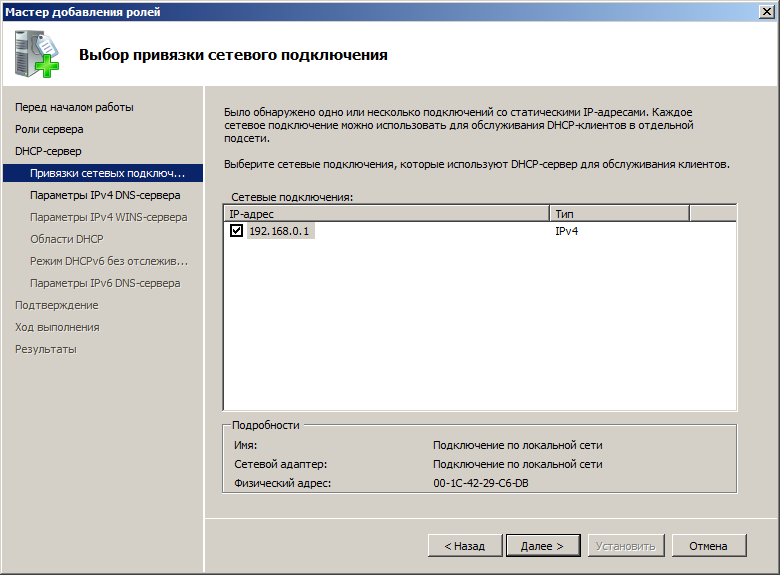
\includegraphics[scale=0.6]{ws2k8/dhcp_4.png}}
\caption{Выбор привязки сетевого подключения}
\label{igas18}
\end{figure}
Укажем родительский домен \textit{vsi.com} и основной DNS сервер \textit{192.168.0.1}, а дополнительный оставим пустым. Сейчас мы указали адрес нашего сервера, т.к. в дальнейшем мы будем использовать его в виде DNS сервера.
\begin{figure}[H]
\center{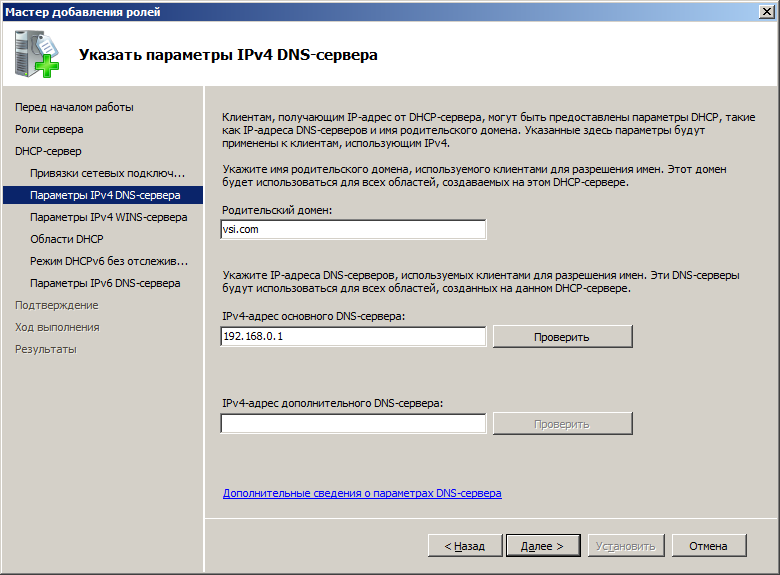
\includegraphics[scale=0.6]{ws2k8/dhcp_5.png}}
\caption{Указать параметры IPv4 DNS-сервера}
\label{igas19}
\end{figure}
На следующем экране выберем \textit{WINS не требуется для приложений в этой сети}, т.к. по сути и функционалу WINS -- DNS для NetBIOS, и использовался в старых версиях Windows и оставлен для совместимости.
\par
На экране \textit{Добавление или изменение DHCP-областей} нажмем на кнопку \textit{Добавить...} и заполним данные как на рисунке \ref{igas22}.
\begin{figure}[H]
\center{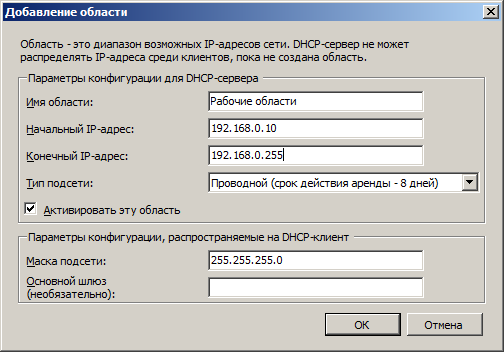
\includegraphics[scale=0.6]{ws2k8/dhcp_8.png}}
\caption{Добавление области}
\label{igas22}
\end{figure}
На следующем экране выберем \textit{Отключить режим без отслеживания состояния DHCPv6 для этого сервера}. Жмем \textit{Далее} затем \textit{Установить}, после завершения установки нажимаем \textit{Закрыть}
\par
Для проверки работоспособности DHCP запустим нашу рабочую станцию на Windows 7, в \textit{настройках подключения по локальной сети} отключим \textit{Протокол Интернета версии 6 (TCP/IPv6)}, а в свойствах \emph{Протокол Интернета версии 4 (TCP/IPv4)} проверим что получение DHCP и DNS происходит автоматически.
\par
Теперь давайте проверим полученные данные, для этого зайдем в \textit{Пуск \DLE Все программы \DLE Стандартные \DLE Командная строка} и введем \texttt{ipconfig /all}. Теперь сравним IPv4-адрес и DNS-сервер с теми которые мы выставили на сервере.
\par
Теперь давайте настроим выдачу IP-адреса по MAC-адресу, для этого запишем наш MAC-адрес(Физический адрес) из только что выведенной информации в \emph{командной строке}.
\par
Теперь на сервере зайдем в \emph{Пуск \DLE Администрирование \DLE DHCP}. Откроем наш сервер \emph{\DLE IPv4 \DLE Рабочие области} и нажмем правой на \emph{Резервирование} и выберем \emph{Создать резервирование...}. Введем \emph{Имя клиента: client, IP-адрес: 192.168.0.20 и MAC-адрес (тот который мы записали на клиентской машине)}.
\par
На рабочей станции зайдем в \emph{Панель управления \DLE Сеть и Интернет \DLE Сетевые подключения} в контекстном меню подключения по локальной сети нажмем \emph{Отключить}, а потом \emph{Включить}.
\par
Теперь давайте проверим полученные данные, для этого зайдем в \textit{Пуск \DLE Все программы \DLE Стандартные \DLE Командная строка} и введем \texttt{ipconfig /all}. Теперь сравним IPv4-адрес и DNS-сервер с теми которые мы выставили на сервере.
\newpage
\subsection{DNS}
Теперь давайте добавим еще одну роль нашего сервера -- DNS. Из \textit{окна начальной настройки} (рис.~\ref{igas12}) в разделе \textit{Настроить этот сервер} нажмем на \textit{Добавить роли}.
\par
В окне \textit{мастера добавления ролей} нажимаем \textit{далее}, чтобы пропустить раздел \textit{Перед началом работы}, и увидим раздел \textit{Выбор ролей сервера} (рис.~\ref{igas16}), отметим \textit{DNS-сервер} и нажмем \textit{Далее}, увидим описание роли и еще раз нажмем \textit{Далее}, затем \emph{Установить}, а потом \emph{Закрыть}.
\par
На сервере зайдем в \emph{Пуск \DLE Администрирование \DLE DNS}. В меню зайдем в пункт \emph{Действие \DLE Создать новую зону...}.
\par
Щелкните на кнопку \emph{Далее} и в следующем окне мастера выберите \emph{Основная зона}, потом выберите \emph{Зону прямого просмотра}, введите имя зоны - \emph{vsi.com}, файл зоны можно оставить по умолчанию, в целях безопасности \emph{запретим динамические обновления}, нажмем \emph{Готово}.
\par
Войдем в нашу зону как показанно на рисунке \ref{dnsi1}, кликнем по ней правой кнопкой мыши и выберем \emph{Создать узел (A или AAAA)...} и заполним как показанно на рисунке \ref{dnsi2}
\begin{figure}[H]
\center{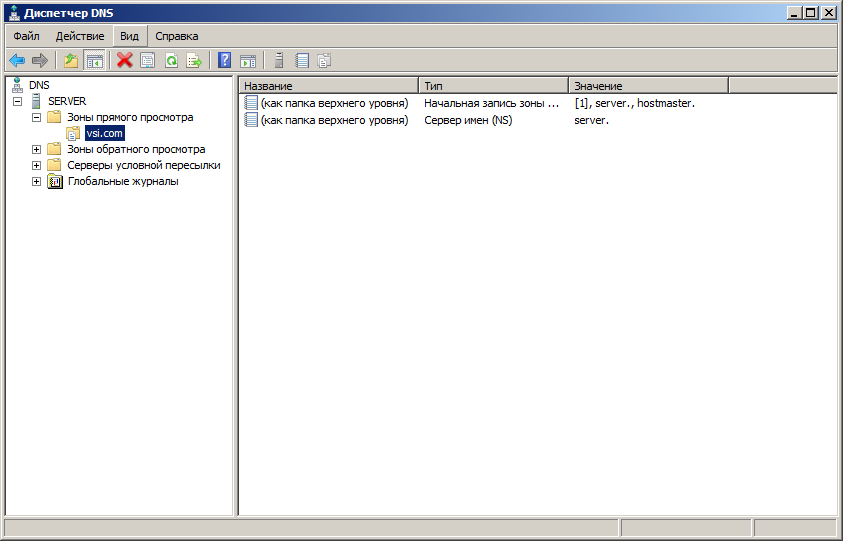
\includegraphics[scale=0.6]{ws2k8/dns_1.png}}
\caption{Диспетчер DNS}
\label{dnsi1}
\end{figure}
\begin{figure}[H]
\center{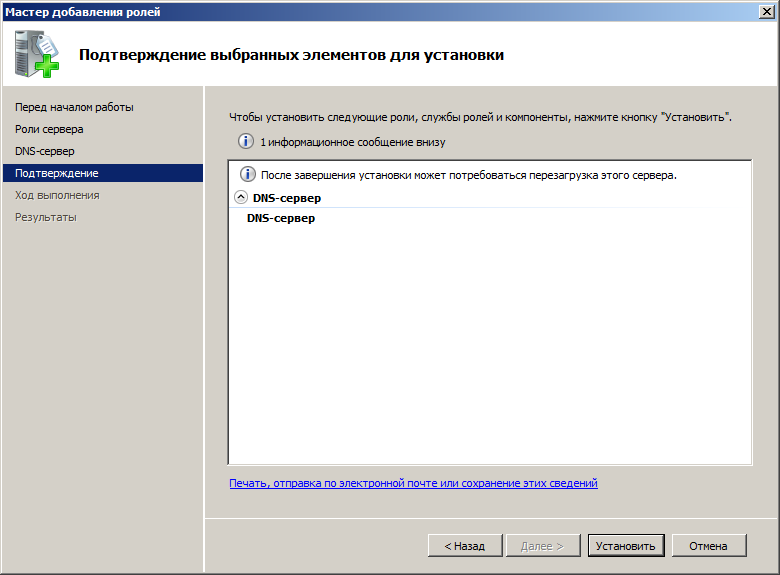
\includegraphics[scale=0.6]{ws2k8/dns_2.png}}
\caption{Диспетчер DNS}
\label{dnsi2}
\end{figure}
На рабочей станции откройте \emph{Командную строку}, для этого зайдем в \textit{Пуск \DLE Все программы \DLE Стандартные \DLE Командная строка} и введем \texttt{ping server.vsi.com}. Если обмен пакетами прошел без потерь, то настройка прошла успешно.
\par
Если Вы захотите сделать домен для рабочей станции, то сначала добавте зарезервированный адрес для нее в DHCP и только потом к этому адресу привязывайте домен.
\cleardoublepage
% Разделы в части II снова начинаются с 1
%\setcounter{section}{0}
\part{Novell Open Enterprise Server 2}
Novell OES2 представляет собой законченное решение по предоставлению базовых сетевых сервисов - регистрация пользователей в сети, сетевая печать, порталы доступа и управления. OES2 может заменить собой любую из существующих систем на базе Linux/Netware/Windows, а присутствующий инструменты миграции обеспечат плавную миграцию данных. Решение построено на базе открытой платформы SUSE Linux Enterprise Server 10 (SLES10) с добавлением функционала коммерческих сервисов Novell. Весомым преимуществом решения можно назвать его высокую степень интегрированности и веб-ориентированности. Управления сетью OES2 сильно проще и удобнее чем даже Windows, а гибкость настройки не ниже чем у любой Linux-системы.

\section{Получение дистрибутива}
Как уже говорилось, решение построено на базе SLES10. Соответственно для установки нам в первую очередь потребуется этот дистрибутив. Дополнительные сервисы вынесены в отдельный диск, функционально являющийся Add-on для SLES10.\par
Чтобы скачать все необходимые пакеты необходимо зарегистрироваться на портале www.novell.com (регистрация бесплатна).\par
Последнюю версию OES2 можно найти на странице novell.com\footnote{http://www.novell.com/products/openenterpriseserver/}. Для установки потребуется скачать SLES10 (32 или 64-битную платформу). Плюс к этому скачиваем диск начинающийся на OES2 (соответственно выбранной платформе).
\clearpage

\section{Установка}
Начало установки.\par
Установка начинается с загрузки сервера с диска SLES10 DVD1. Диск с сервисами OES2 пригодится несколько позже, во время настройки. Если загрузка удалась, то вы увидите следующее окно. (рис.~\ref{fig1})
\begin{figure}[H]
\center{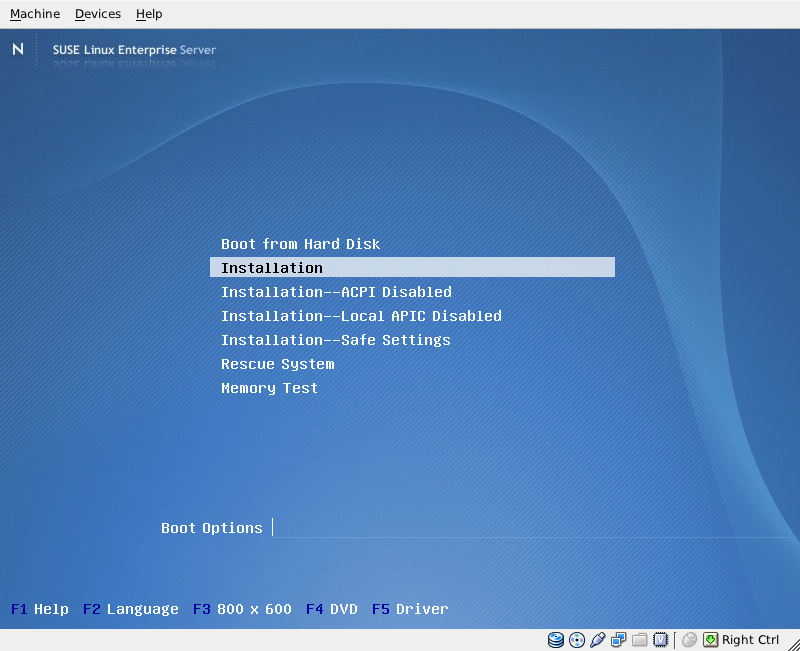
\includegraphics[width=1\linewidth]{oes/1.png}}
\caption{Начало установки}
\label{fig1}
\end{figure}
По умолчанию выбран пункт <<Boot from Hard Disk>> (Загрузка с жёсткого диска). Для начала установки выбираем пункт <<Installation>>.
\clearpage

Первое окно — выбор языка установки, выбираем <<Русский>>, нажимаем <<Применить>>. (рис.~\ref{fig2})
\begin{figure}[H]
\center{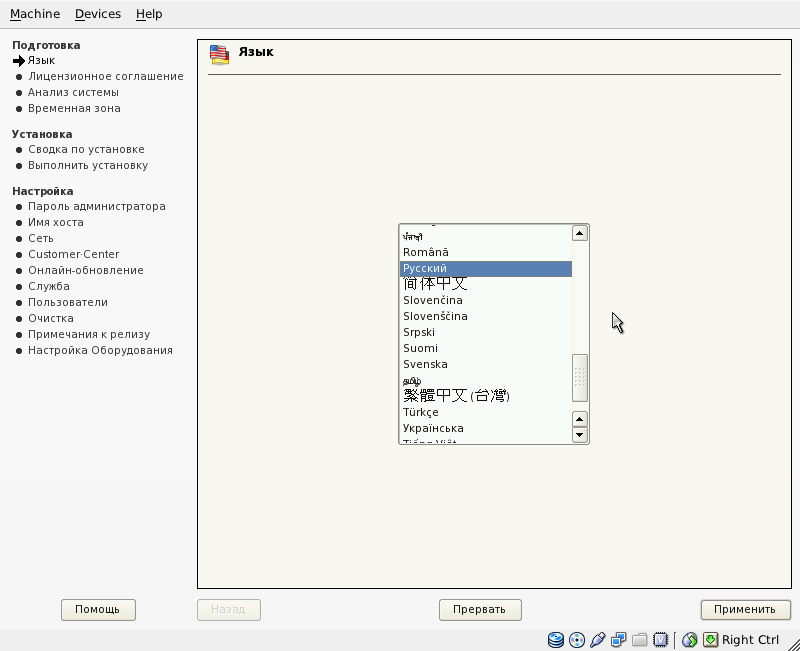
\includegraphics[width=1\linewidth]{oes/2.png}}
\caption{Выбор языка}
\label{fig2}
\end{figure}
\clearpage

Далее предлагается принять лицензию на SLES10 <<Да, я согласен с условиями лицензионного соглашения>>, без чего дальнейшая установка невозможна. (рис.~\ref{fig3})
\begin{figure}[H]
\center{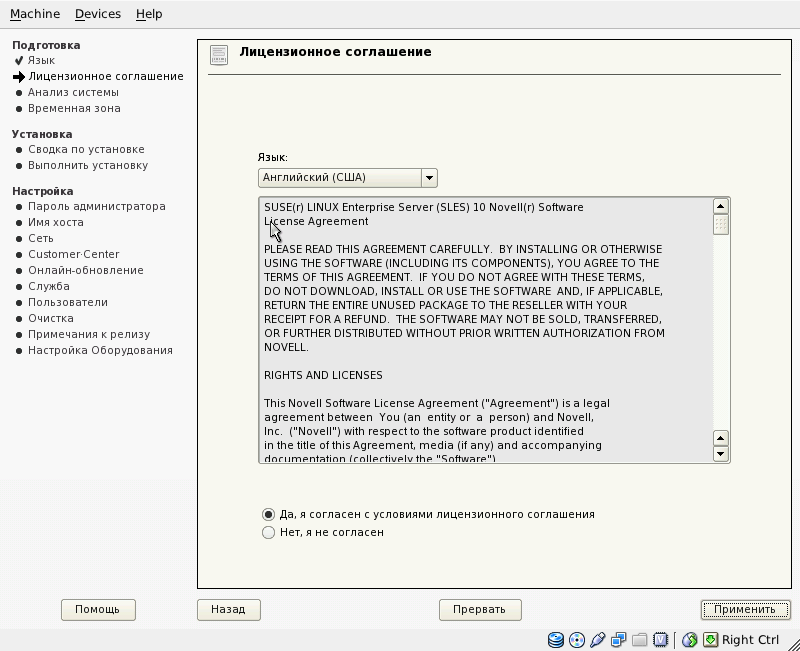
\includegraphics[width=1\linewidth]{oes/3.png}}
\caption{Лицензионное соглашение}
\label{fig3}
\end{figure}
\clearpage

Установщик автоматически предлагает вариант <<Новая установка>>. Если бы на сервере была установлена какой-либо SUSE Linux, то был бы доступен выбор варианта обновления. (рис.~\ref{fig4})
\begin{figure}[H]
\center{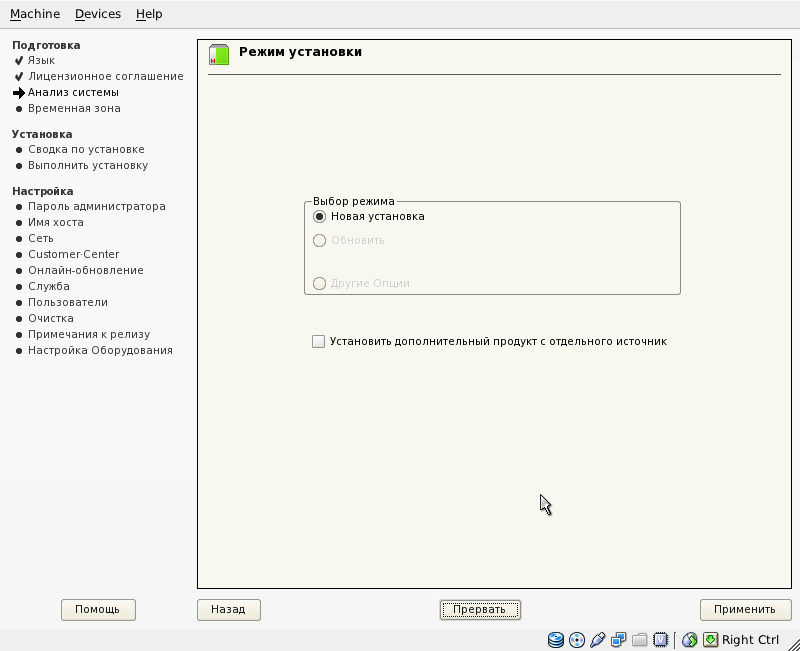
\includegraphics[width=1\linewidth]{oes/4.png}}
\caption{Выбор режима установки}
\label{fig4}
\end{figure}
\clearpage

После выбора временной зоны появляется итоговая сводка. Это последний этап конфигурирования системы перед установкой. На последующих шагах для настройки NSS\footnote{Novell Storage Services (NSS) - файловая система, используемая в Novell для создания томов на файловом сервере} нам потребуется свободное дисковое пространство. Для этого можно выделить отдельный жесткий диск (или же поднять для этих целей отдельностоящий сервер). В нашем случае мы переразобъём текущий раздел, выделив свободное место на нём.
\begin{figure}[H]
\center{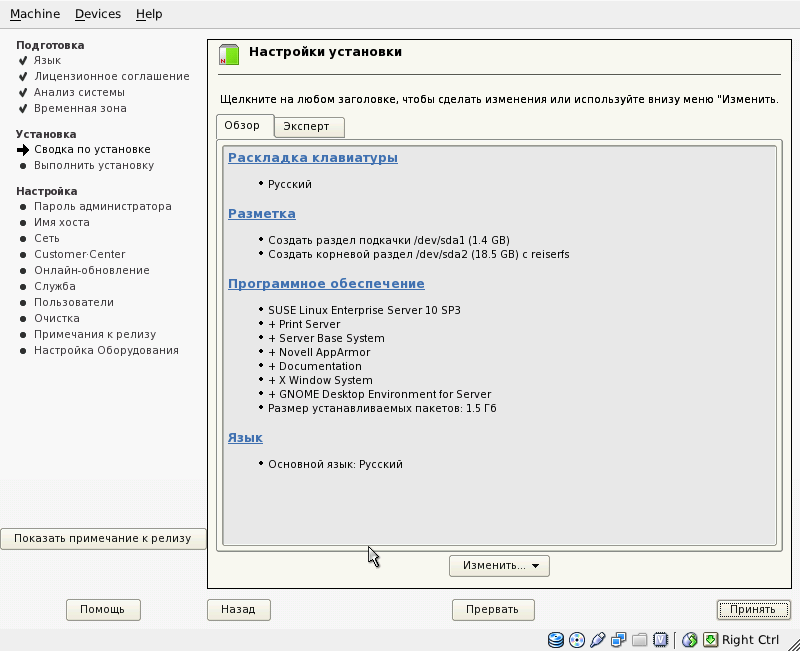
\includegraphics[width=1\linewidth]{oes/p1.png}}
\caption{Сводка установки}
\label{p1}
\end{figure}
Заходим в раздел <<Разметка>>.
\clearpage

Полностью переделывать разметку мы не будем, поэтому выбираем пункт <<Настроить раздел согласно предложению>>.
\begin{figure}[H]
\center{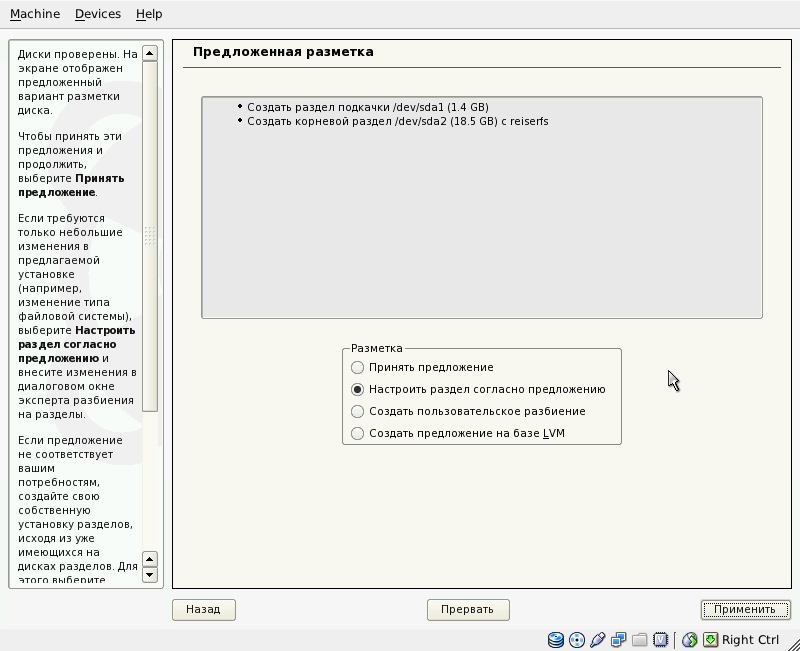
\includegraphics[width=1\linewidth]{oes/p2.png}}
\caption{Предложенная разметка}
\label{p2}
\end{figure}
\clearpage

Здесь мы уменьшим основной раздел нажав кнопку <<Изменить размер>>.
\begin{figure}[H]
\center{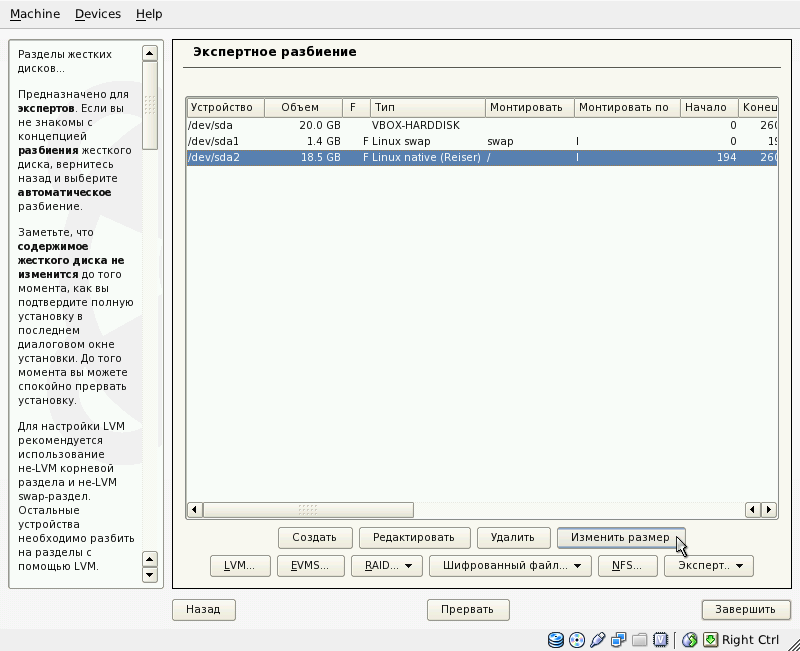
\includegraphics[width=1\linewidth]{oes/p3.png}}
\caption{Изменение разметки}
\label{p3}
\end{figure}
\clearpage

Отрезаем часть от раздела. В будущем мы используем это свободное пространство для создания NSS томов.
\begin{figure}[H]
\center{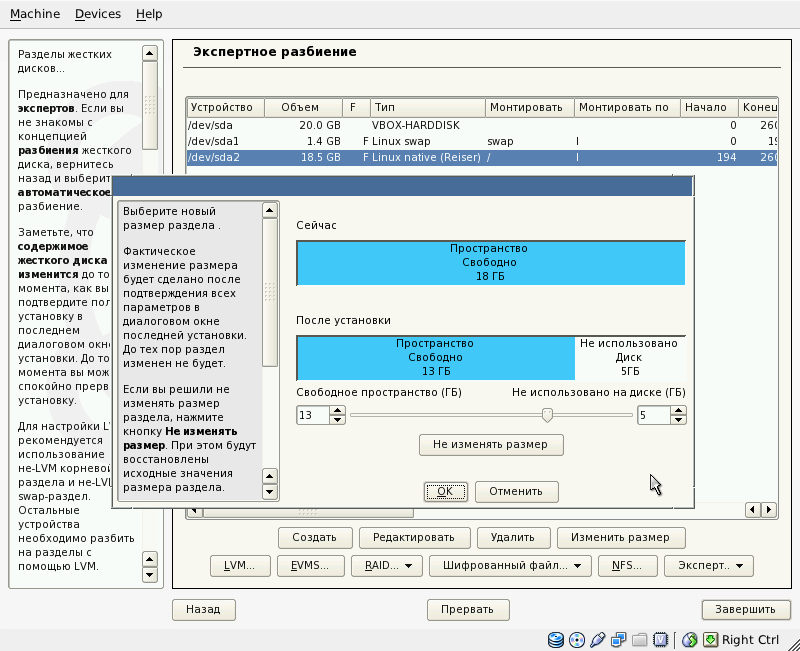
\includegraphics[width=1\linewidth]{oes/p4.png}}
\caption{Изменение разметки}
\label{p4}
\end{figure}
\clearpage

Теперь у нас появилось немного свободного дискового пространства, можно приступать к установке, нажав <<Принять>>. (рис.~\ref{p5})
\begin{figure}[H]
\center{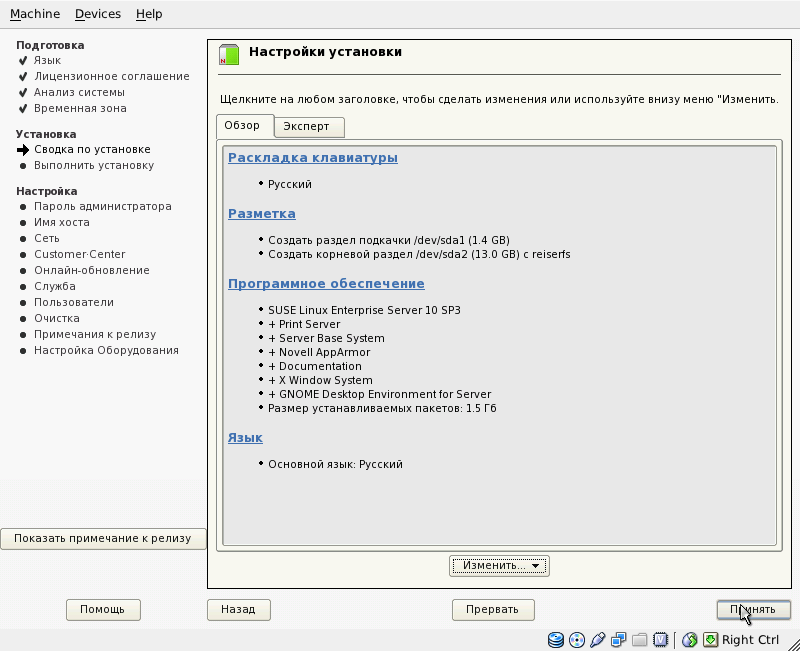
\includegraphics[width=1\linewidth]{oes/p5.png}}
\caption{Сводка установки}
\label{p5}
\end{figure}
\clearpage

После перезагрузки мы можем приступить к первоначальной настройке сервера.\\
Начинаем с пароля администратора root. Если пароль указать недостаточно стойким или присутствующим в базе типовых паролей, то система выдаст предупреждение о потенциальной угрозе. (рис.~\ref{fig6})
\begin{figure}[H]
\center{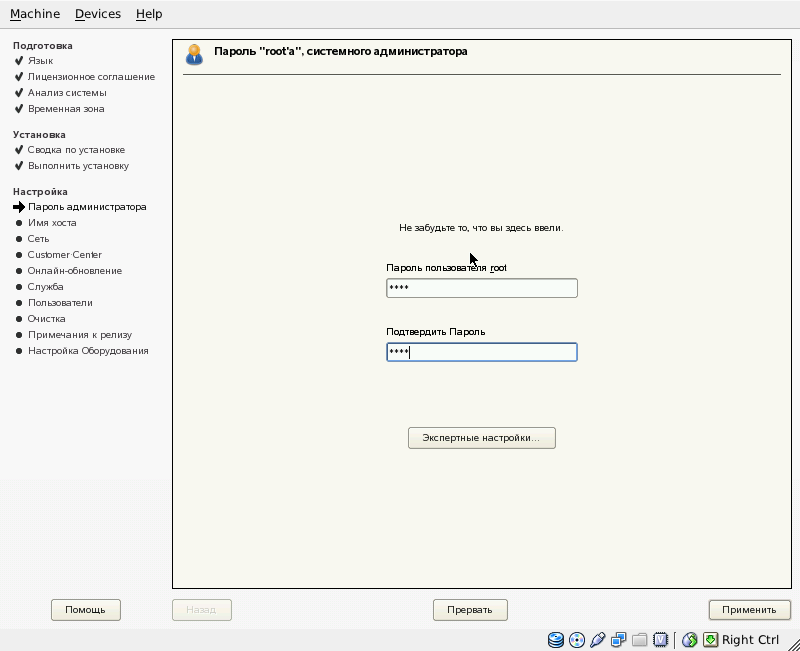
\includegraphics[width=1\linewidth]{oes/rootpasswd.png}}
\caption{Пароль системного администратора}
\label{fig6}
\end{figure}
\clearpage

Следующий этап это указание имени узла (в нашем случае oes2 - по названию операционной системы) и домена DNS (вариации на тему <имя компании>.ru). (рис.~\ref{fig7})
\begin{figure}[H]
\center{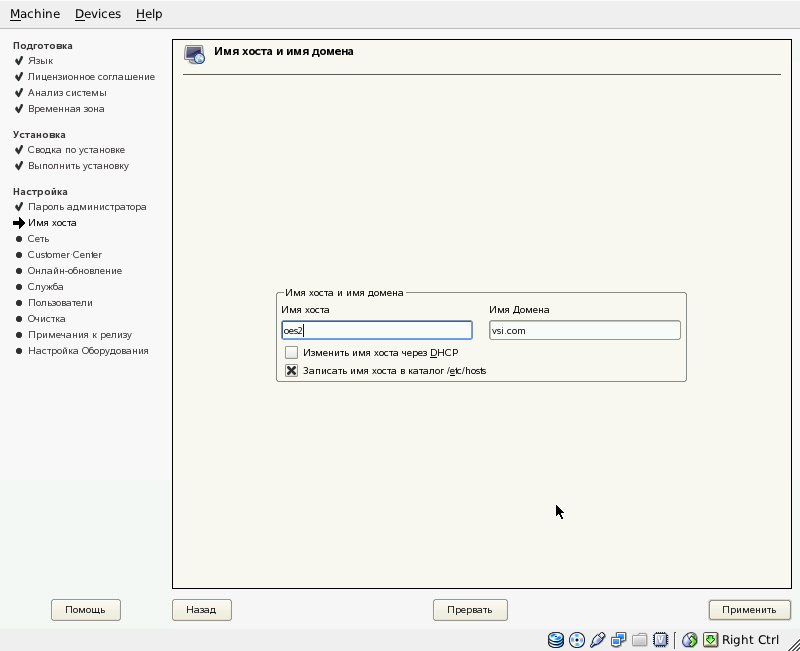
\includegraphics[width=1\linewidth]{oes/7.png}}
\caption{Имя хоста и имя домена}
\label{fig7}
\end{figure}
\clearpage

В разделе <<Настройка сети>> необходимо задать ip адрес сервера. По умолчанию сетевые адаптеры не настроены, либо настроены на использование DHCP, что совершенно не годится в случае с сервером. Для этого нажимаем <<Изменить>> и выбираем <<Сетевые интерфейсы>> (рис.~\ref{figNetworkall})
\begin{figure}[H]
\center{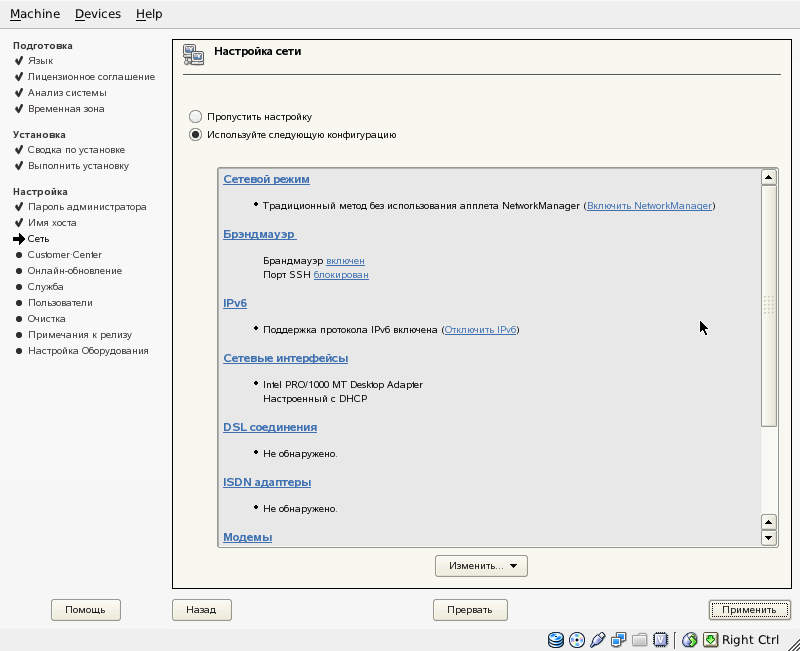
\includegraphics[width=1\linewidth]{oes/networkall.png}}
\caption{Настройка сети}
\label{figNetworkall}
\end{figure}
\clearpage

Сетевую карту необходимо настроить на статическое получение адреса — выбрать <<Установка статического адреса>> и задать все необходимые параметры: IP-адрес и маску подсети.
\begin{figure}[H]
\center{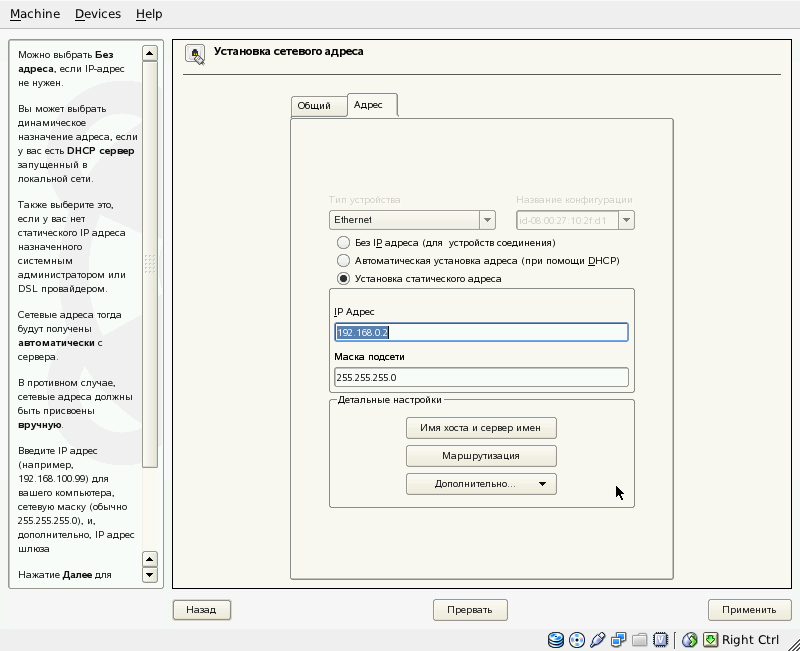
\includegraphics[width=1\linewidth]{oes/8.png}}
\caption{Настройка сетевого адреса}
\label{fig8}
\end{figure}
\clearpage

Следующим шагом будет настройка DNS. Жмём <<Имя хоста и сервер имён>> и прописываем наш сервер в <<Сервер имён 1>>. Завершаем настройку кнопкой <<Применить>>. (рис.~\ref{fig9})
\begin{figure}[H]
\center{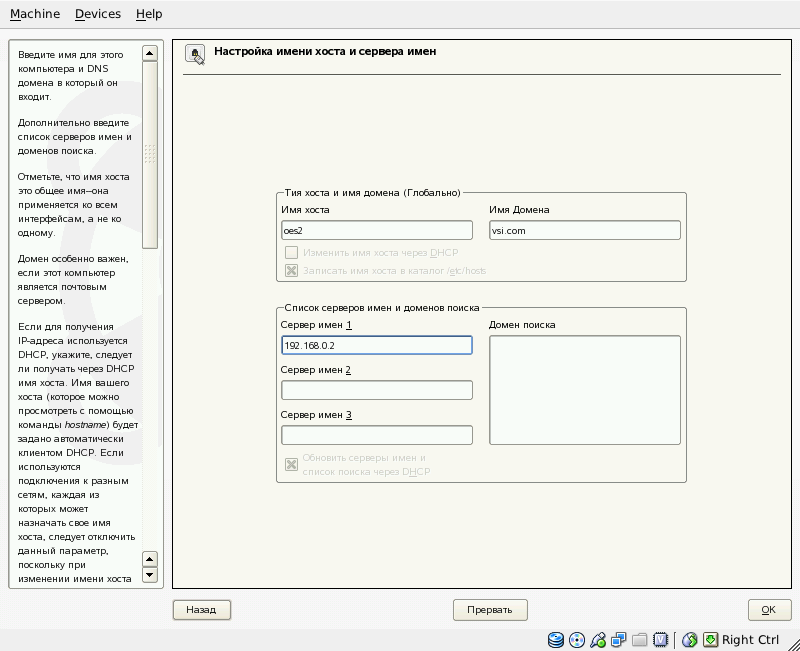
\includegraphics[width=1\linewidth]{oes/9.png}}
\caption{Настройка DNS}
\label{fig9}
\end{figure}
\clearpage

Теперь, когда сеть настроена, можно попробовать подключиться к сети Интернет и проверить последние обновления с сайта novell.com. (рис.~\ref{fig10})
\begin{figure}[H]
\center{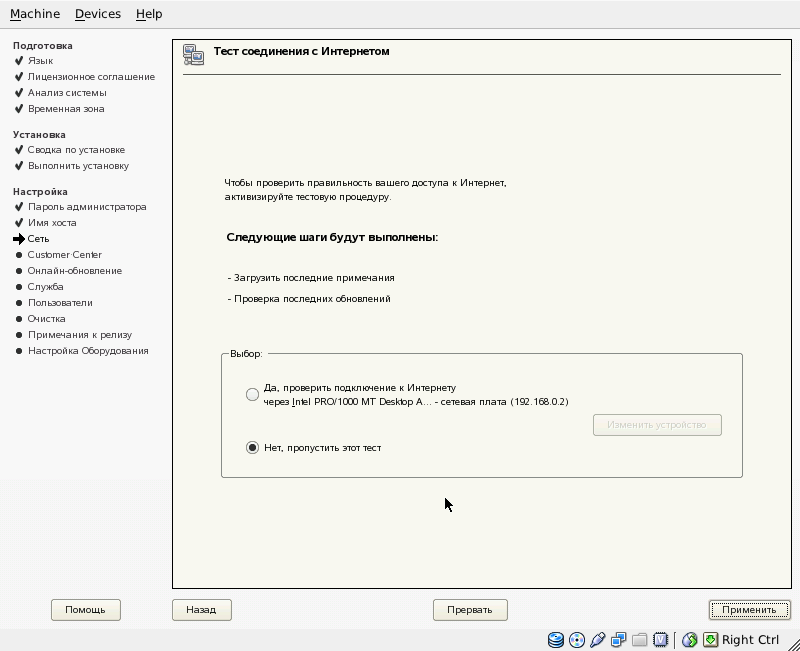
\includegraphics[width=1\linewidth]{oes/10.png}}
\caption{Тест соединения с Интернетом}
\label{fig10}
\end{figure}
Если на текущем этапе нет желания или возможности проверить подключение к сети Интернет, то выбираем вариант <<Нет, пропустить этот тест>>.
\clearpage

Добавить скрин с сертификатом.
\clearpage

Ещё один тонкий момент, требующий внимания — настройка сертификата сервера. Как видно исходное значения поля <<Страна>> выставлено равным <<RU.KOI8-R>>, что не совсем правильно. Чтобы изменить параметры сертификата жмём линк <<Управление СА>>. В открывшемся окне находим кнопку <<Редактировать Установки по Умолчанию>> и меняем поле страна на Россия. (рис.~\ref{fig11})
\begin{figure}[H]
\center{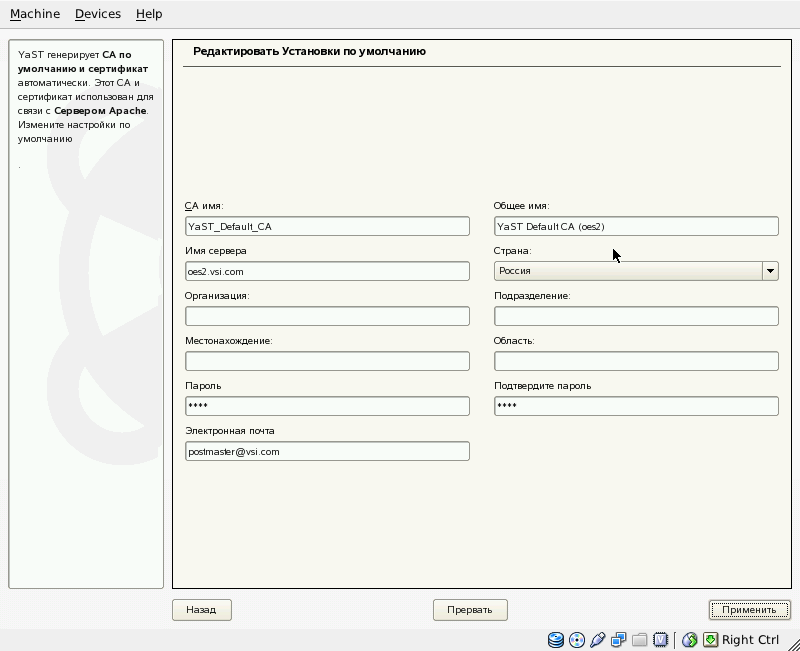
\includegraphics[width=1\linewidth]{oes/11.png}}
\caption{Редактирование CA сертификата}
\label{fig11}
\end{figure}
\clearpage

Следующий этап это создание локальных пользователей. (рис.~\ref{fig12})
\begin{figure}[H]
\center{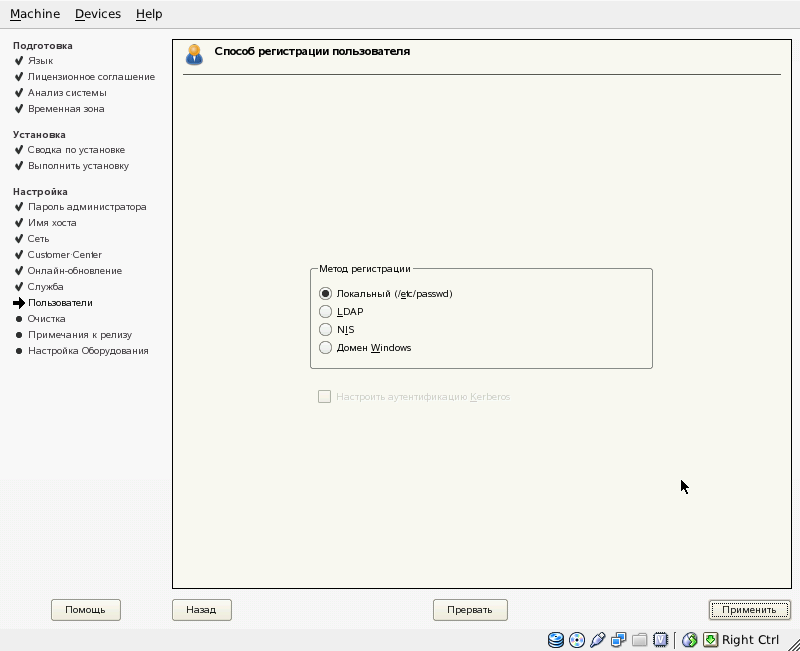
\includegraphics[width=1\linewidth]{oes/12.png}}
\caption{Способ регистрации пользователей}
\label{fig12}
\end{figure}
Выбираем метод регистрации <<Локальный (/etc/passwd)>>.
\clearpage

Произвольно задаём имя пользователя и пароль. (рис.~\ref{fig13})
\begin{figure}[H]
\center{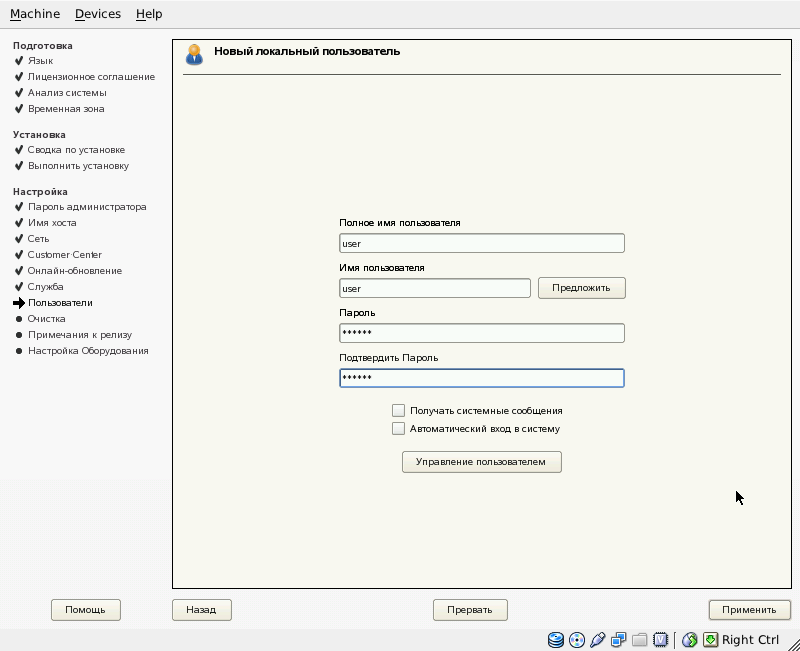
\includegraphics[width=1\linewidth]{oes/13.png}}
\caption{Создание локального пользователя}
\label{fig13}
\end{figure}
Жмём кнопку <<Применить>>, переходим к окну примечаний к выпуску и вновь жмём кнопку <<Применить>>.
\clearpage

Окно настройки оборудования показывает текущие настройки видеокарты, принтеров и звука. Оставляем всё без изменений. (рис.~\ref{fig14})
\begin{figure}[H]
\center{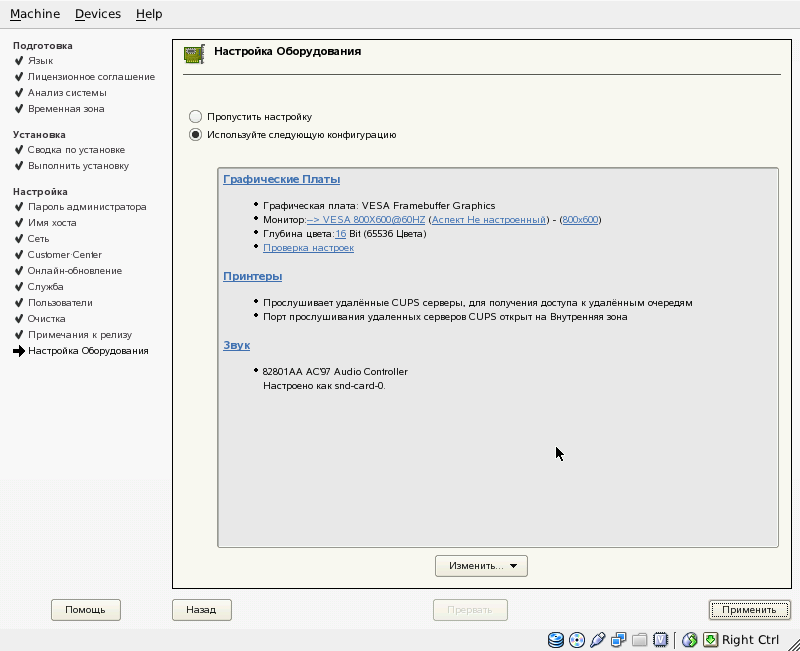
\includegraphics[width=1\linewidth]{oes/14.png}}
\caption{Настройка оборудования}
\label{fig14}
\end{figure}
\clearpage

Установка завершена, о чём нам и сообщает открывшееся окно. (рис.~\ref{fig15})
\begin{figure}[H]
\center{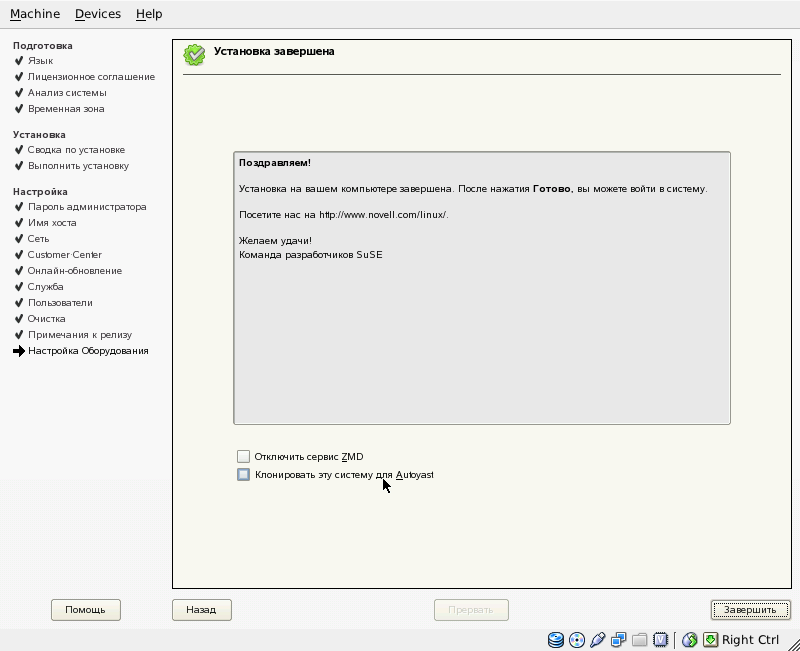
\includegraphics[width=1\linewidth]{oes/15.png}}
\caption{Завершение установки}
\label{fig15}
\end{figure}
Если мы хотим сохранить настройки для будущего клонирования операционной
системы, то ставим крестик в поле <<Клонировать эту систему для Autoyast>>. Жмём кнопку <<Завершить>>.
\clearpage

Теперь мы можем зайти на сервер локально и закончить настройку сервера. (рис.~\ref{fig16})
\begin{figure}[H]
\center{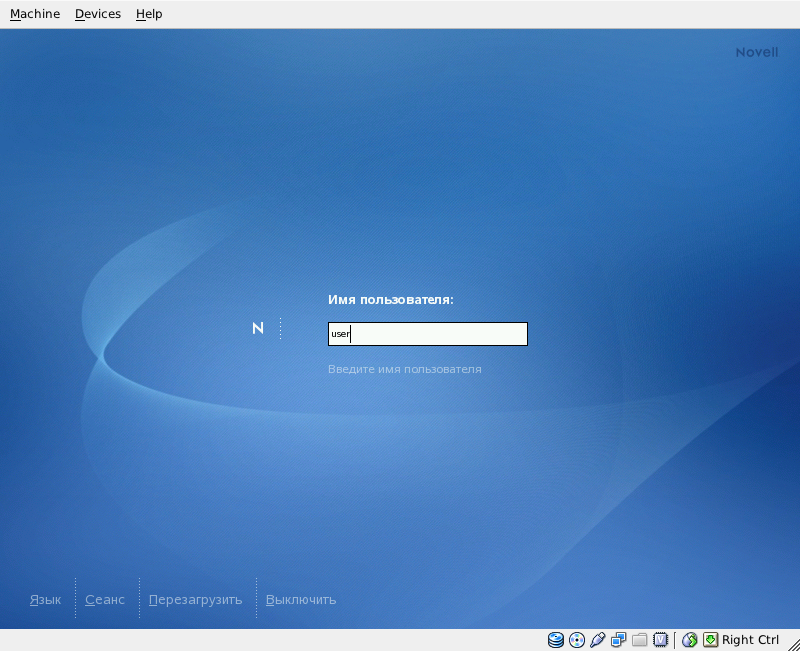
\includegraphics[width=1\linewidth]{oes/16.png}}
\caption{Вход в систему}
\label{fig16}
\end{figure}
\clearpage

\section{Настройка DHCP}
Open Enterprise Server основывается на linux дистрибутиве openSUSE\footnote{http://www.opensuse.org/ru/}, поэтому по вопросам использования или настройки можно воспользоваться любыми справочными материалами, посвящёнными этому дистрибутиву. Здесь мы коснёмся лишь настройке сервисов, относящихся к диску OES2.\par 
Все настройки ОС openSUSE пройзводятся с помощью менеджера YaST\footnote{http://ru.opensuse.org/YaST}.
\begin{figure}[H]
\center{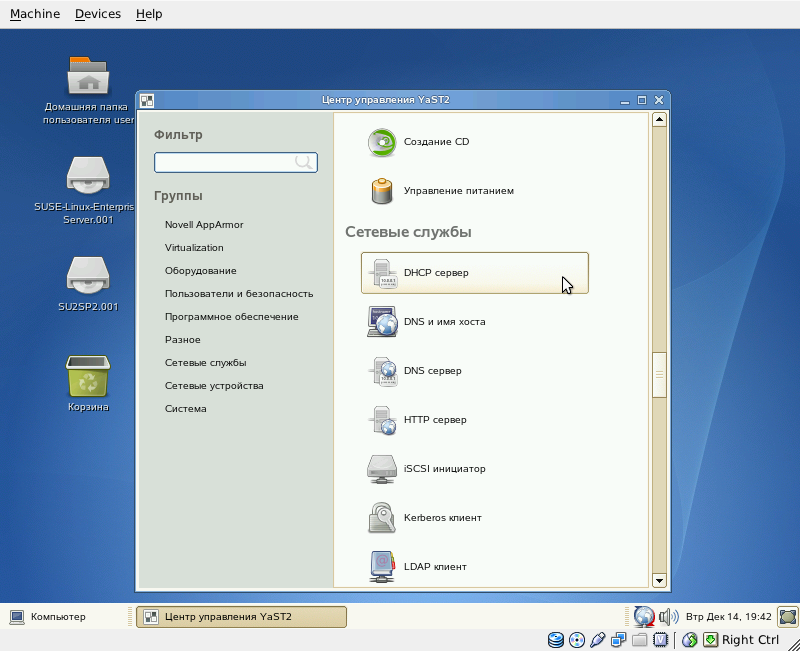
\includegraphics[width=1\linewidth]{oes/yast.png}}
\caption{YaST}
\label{yast}
\end{figure}
Настройка DHCP здесь ничем принципиально не отличается от настройки в Windows системах. Выбирается сетевой интерфейс, на котором будут раздаваться IP адреса, также назначаются сервера имён и диапазон IP адресов. Последний шагом станет выбор, будет ли сервер стартовать при загрузке операционной системы или его следует запускать вручную.\par
В процессе настройки у системы может возникнуть желание доустановить недостающие компоненты. Для этого необходимо вставить соответствующий диск с ПО. Базовые пакеты находятся на дисках SLES, в то время как всё проприетарное программное обеспечение лежит на диске OES2.

\section{Настройка eDirectory}
Настройка eDirectory\footnote{http://www.novell.com/russia/products/edirectory/}

\section{Настройка клиента}
Установка Novell Client\footnote{http://www.novell.com/products/clients/}
\cleardoublepage	
%\setcounter{section}{0}
\part{Теоретические сведения}
\newpage
\end{document}